\chapter{Trabajo Previo}


El presente capítulo aborda los estudios más relevantes hasta la fecha relacionados con la detección de emociones en el texto, los modelos de aprendizaje automático utilizados en dicha tarea y su aplicación en el contexto de las redes sociales.

Se mencionan estudios que se centran en la detección de opiniones negativas o positivas en textos en distintos dominios, como las calificaciones de películas. Se destaca la importancia que ha tenido en este campo contar con una base de términos clasificados según su orientación emocional, lo cual permite realizar análisis automáticos. Además, se explora la evolución hacia el uso de redes neuronales, específicamente modelos basados en la arquitectura Transformer, como BERT, para capturar el sentido y las relaciones entre palabras en el análisis de texto. También se discute la aplicación de estos modelos en español. Por último, se aborda el análisis de sentimientos y emociones en redes sociales como blogs y Twitter, resaltando su utilidad en la comprensión de la percepción pública y en la identificación de estados emocionales en torno a eventos políticos y sociales.


\section{Aprendizaje supervisado en la detección de emociones}



La detección automática de las respuestas internas que las personas reflejan en el texto ante ciertos fenómenos ha sido estudiada con mucho interés. Así lo establecieron \cite{pang2002thumbs}, quienes destacaron la importancia de desarrollar sistemas capaces de identificar si existe opinión negativa o positiva ante textos que reflejen opiniones subjetivas. Para este propósito, se empleó el dominio de las reseñas en línea de películas, lo que facilita la tarea de construir algoritmos de aprendizaje supervisado, al contar con una clasificación negativa o positiva del texto por parte del usuario. Estos algoritmos buscan entrenar un modelo a partir de ejemplos previamente clasificados, que sea capaz de predecir una variable objetivo dadas unas variables predictoras. En ese sentido, las variables predictoras se construyen a partir del texto, principalmente mediante la elaboración de unigramas, que son elementos individuales del texto, como las palabras, y como variable objetivo se utiliza la clasificación asignada. Por otro lado, \cite{turney2002thumbs} intentó establecer mediante aprendizaje no supervisado si una determinada reseña en línea sobre diversos temas presenta un sentimiento negativo o positivo. Para ello, utiliza el concepto de orientación semántica presentado por \cite{hatzivassiloglou1997predicting} para determinar si una frase tiene una orientación negativa o positiva, y así poder decidir si la reseña en su conjunto es positiva o negativa. En general, la determinación de la orientación negativa o positiva dentro del texto constituye la detección de la polaridad.

Para llevar a cabo la detección automática de los estados emocionales presentes en el texto, ha sido importante contar con un corpus de términos que cuenten con una clasificación previa. En este sentido, \cite{strapparava2004wordnet} realizaron una anotación manual de los estados emocionales usando las categorías desarrolladas por \cite{ortony1987referential}, de los términos encontrados en WordNet, una base de datos de términos en inglés agrupados en grupos de sinónimos y con relaciones semánticas entre grupos creada por \cite{miller1995wordnet}. A partir de las anotaciones manuales de las emociones de ciertos términos presentes en la base, se estableció la categoría emocional de nuevos términos gracias a los sinónimos y las relaciones semánticas, construyendo así una base de datos de estados emocionales llamada WordNet-Affect. En esta misma línea, \cite{wiebe2005annotating} elaboraron una anotación manual de los estados emocionales presentes en las oraciones de un gran volumen de noticias, teniendo en cuenta el contexto.

En el contexto de la clasificación automática de las emociones en el texto, \cite{alm2005emotions} utilizaron los cuentos infantiles para desarrollar un modelo de aprendizaje supervisado capaz de detectar emociones en las frases. Para ello, se elaboró una anotación manual de estas frases que constituyen la base de datos y, posteriormente, se generó un conjunto de features para dichas frases que se utilizaron para entrenar un clasificador lineal




\section{Redes neuronales para el análisis de texto}

Las técnicas tradicionales de análisis de emociones en el texto han estado principalmente basadas en la relación que existe entre los términos que conforman el texto y un estado emocional determinado. Aunque este tipo de análisis ha sido de gran utilidad, no posee la capacidad de tener en cuenta el sentido, es decir, la relación que existe entre las palabras que componen el texto, además del orden en que se presentan. Debido a esto, recientemente el campo de estudio ha migrado hacia el uso de algoritmos capaces de captar esta relación contextual, específicamente las redes neuronales.

Con el objetivo de resumir el estado del arte, \cite{acheampong2021transformer} realizaron un recuento de las distintas arquitecturas de redes neuronales utilizadas recientemente para esta tarea, incluidas las RNN (redes neuronales recurrentes), que fueron popularizadas entre otros, por \cite{cho2014learning}. Estas redes tienen una arquitectura adecuada para datos secuenciales, como las tareas de NLP. Son una estructura autoregresiva, generando la salida del paso t+1 con base en la entrada en el tiempo t+1 y la salida en el tiempo t. Sin embargo, debido a su arquitectura, la optimización de los pesos que conforman la topología de las RNN se vuelve compleja para el cálculo del gradiente del error, ya que se debe pasar tantas veces por los pesos de la red como pasos en el tiempo existan (como el número de caracteres en una palabra), lo que hace difícil computar secuencias particularmente largas dada la carencia de paralelizacion del calculo.

Aunque las RNN permiten preservar de alguna manera la relación contextual del texto al tener una estructura secuencial, esta impide la paralelización de su cómputo, ya que se requieren las salidas de ejemplos anteriores para realizar el siguiente paso en el tiempo. Además, debido a este funcionamiento secuencial, si hay un gran número de pasos en el tiempo, es poco probable que la red considere para un punto muy adelante, información presente al inicio. Para abordar estos inconvenientes, \cite{vaswani2017attention} desarrollaron los Transformers, una arquitectura en la que los datos de entrada se introducen en la red de manera simultánea, como todas las palabras en una frase por ejemplo. Esto se logra a través de una arquitectura definida como auto-atención. La auto-atención permite que una red utilice información de textos arbitrariamente largos de manera eficiente, ya que para cada elemento en la entrada, el modelo accede a todas las entradas hasta ese elemento. Además, el cálculo para cada elemento es independiente de los demás cálculos. Esto posibilita que la representación de cada dato, en este caso cada palabra, considere su importancia con respecto las demás palabras en la oración. Esta transformación, aplicada tanto a los datos de entrada como a los de salida, se emplea para entrenar los pesos de la red. De esta manera, la red puede procesar datos de manera simultánea y tener en cuenta toda la información disponible. Un esquema de esta arquitectura se puede apreciar en la Figura \ref{figure:transformers}.

\begin{figure}[!htbp]
	\centering
	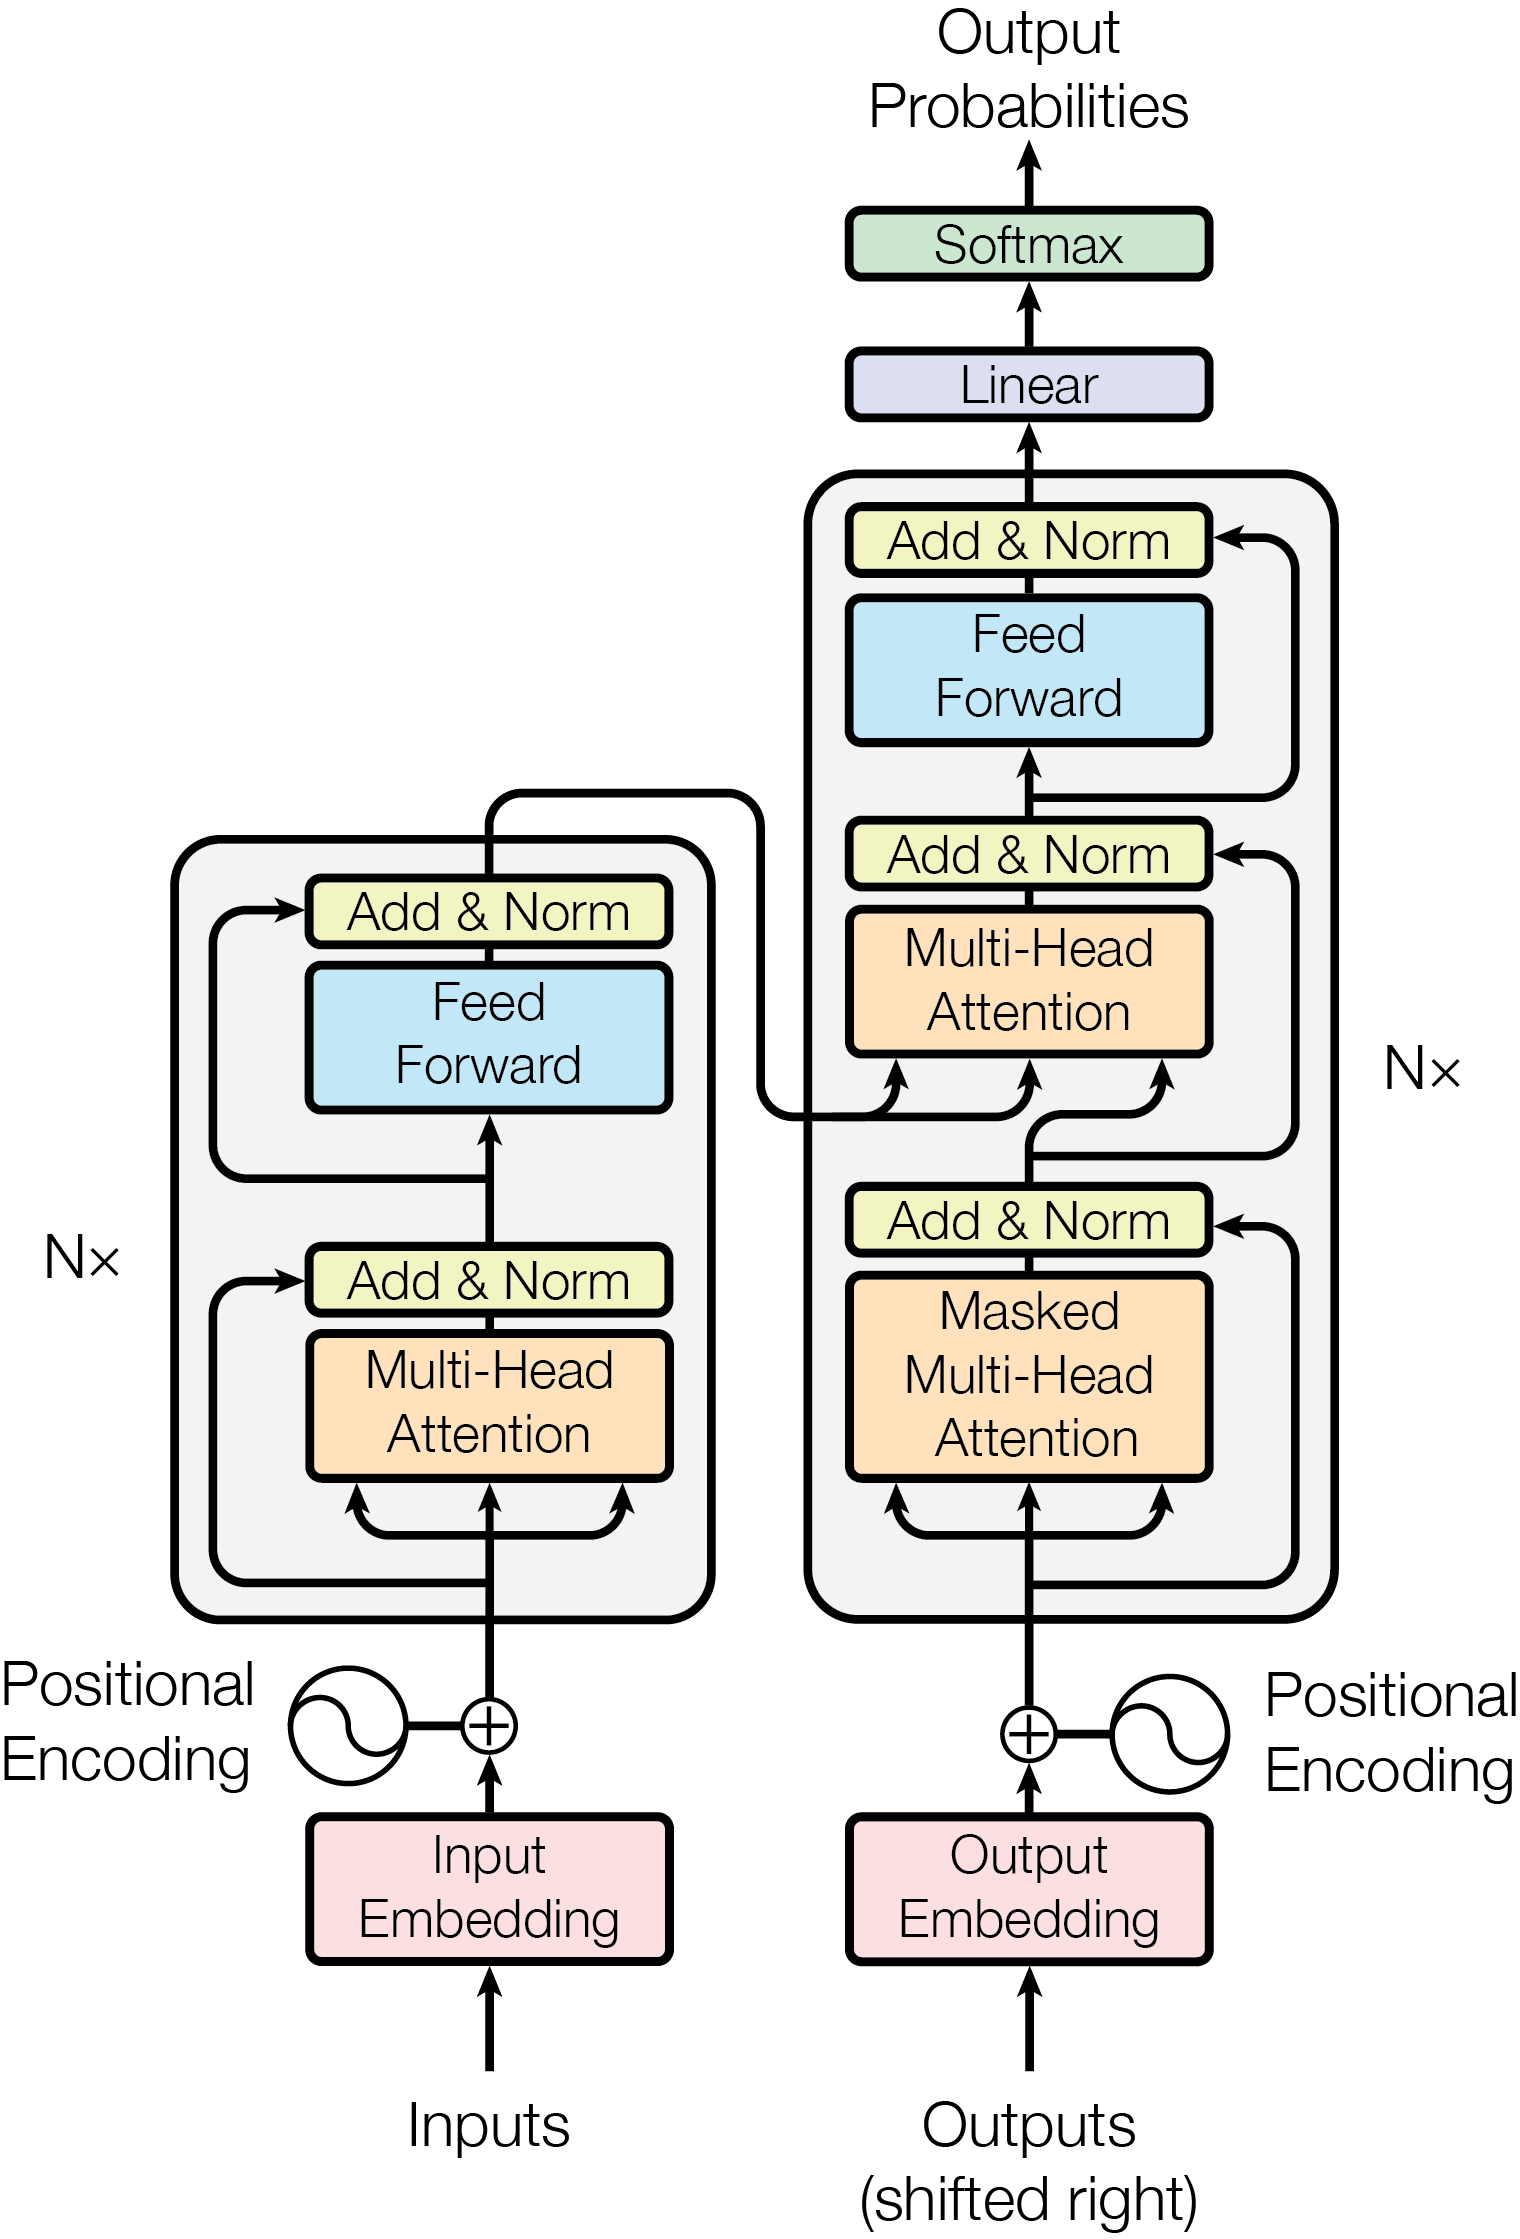
\includegraphics[scale=0.15]{Images & Logos/Transformers.png} 
	\caption{Arquitectura de los Transformers}
	\label{figure:transformers}
\end{figure}

En la figura \ref{fig:comparacion_modelos} se muestra una comparación entre los mecanismos de auto atención de los Transformers y la estructura recurrente de las RNN, en donde se aprecia la manera de calculo simultaneo de una y secuencial de la otra.


\begin{figure}[!htbp]
	\centering
	\begin{subfigure}[b]{0.35\textwidth}
		\centering
		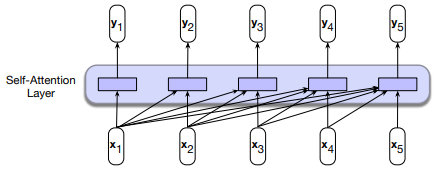
\includegraphics[scale=0.45]{Images & Logos/self-attention.png}
		\caption{Mecanismo de auto-atención de los transformers}
		\label{fig:auto-atencion}
	\end{subfigure}
	\hfill
	\begin{subfigure}[b]{0.52\textwidth}
		\centering
		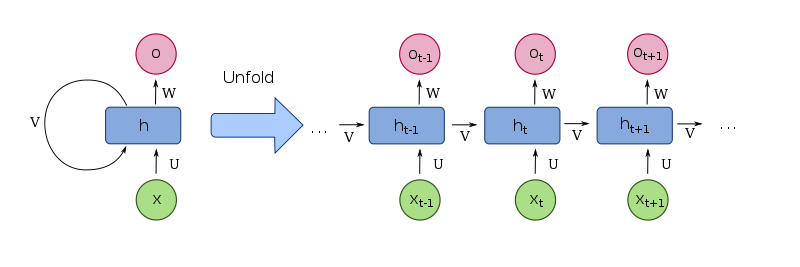
\includegraphics[scale=0.36]{Images & Logos/Recurrent_neural_network_unfold.svg.png}
		\caption{arquitectura de las RNN}
		\label{fig:RNN}
	\end{subfigure}
    \caption{Comparación entre mecanismos de redes. Fuentes \cite{jurafsky2000speech}, \cite{enwiki:1109264340}}
	\label{fig:comparacion_modelos}
\end{figure}




Gracias a la capacidad de paralelización y a la habilidad para conservar la relación entre palabras distantes en el texto que presentan los Transformers, es posible entrenar un modelo de lenguaje con grandes volúmenes de información para así contar con una red de gran poder predictivo. Es precisamente en este contexto que \cite{devlin2018bert} desarrollaron un modelo basado en Transformers, capaz de aprender el sentido del lenguaje de manera general y luego utilizar lo aprendido para diversas tareas de procesamiento de lenguaje natural, denominado BERT (Bidirectional Transformers for Language Understanding). Para esto, se emplea una arquitectura donde las capas de entrada son las representaciones vectoriales de las palabras (Embeddings), y a partir de ahí se incluyen múltiples capas de Transformers. En su proceso de entrenamiento, se suministran dos oraciones consecutivas con palabras faltantes y se asignan dos tareas simultáneas: predecir qué palabra podría ser la faltante y determinar el orden de las oraciones. Esto le permite al modelo aprender del contexto del lenguaje a nivel de palabras, utilizando tanto las que vienen antes como las que vienen después como fuentes de información, y también aprender del contexto de las oraciones al identificar su secuencia. Para ello, se utilizó la totalidad de Wikipedia en su fase de entrenamiento. Una vez preentrenado, este modelo es capaz de utilizar su representación contextual del lenguaje para realizar diversas tareas de procesamiento de lenguaje natural, como análisis de sentimiento. Esto se logra agregando una capa final a la red que genere un posible resultado, por ejemplo, mediante una función softmax que permita asignar probabilidades a distintas clases y luego comparar este resultado con los valores esperados. El esquema de esta arquitectura se puede apreciar en la Figura \ref{figure:BERT}.

\begin{figure}[t]
	\centering
	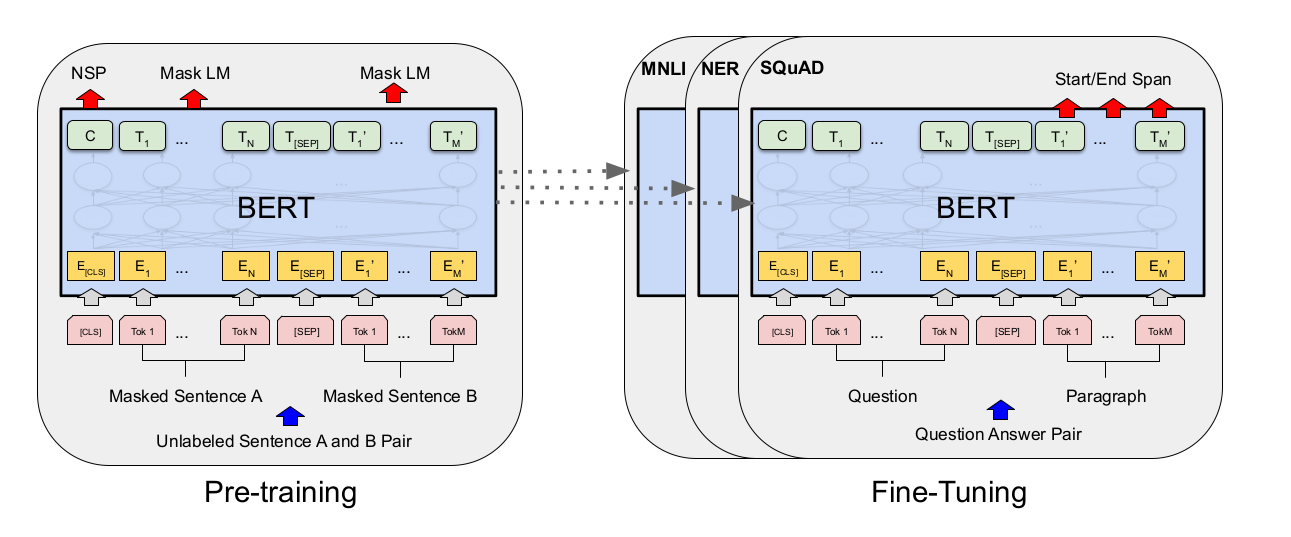
\includegraphics[scale=0.35]{Images & Logos/BERT.png} 
	\caption{Arquitectura de BERT. Fuente \cite{devlin2018bert}}
	\label{figure:BERT}
\end{figure}


En lo que respecta a la aplicación de modelos tipo BERT en español, \cite{canete2020spanish} destacan que hasta la fecha no existía un modelo de este tipo entrenado específicamente para este lenguaje, además del modelo BERT multilingüe. Por esta razón, se propusieron entrenar un modelo destinado al español, utilizando además de la Wikipedia en español, textos provenientes de publicaciones de las Naciones Unidas, gobiernos y charlas TED. El resultado fue un modelo que supera al BERT multilingüe en múltiples tareas de evaluación para el español.



\section{Sentimientos y emociones en redes sociales}

El campo de estudio del análisis de sentimiento del texto en Internet ha cobrado cada vez más importancia,tanto para usuarios individuales como para la industria de la publicidad, el mercado financiero y la academia tal como lo describen \cite{pang2008opinion}. Por lo tanto, los autores realizan un repaso de las distintas técnicas y aplicaciones que consideran relevantes hasta la fecha.

Un ámbito particular donde los usuarios individuales generan grandes volúmenes de información sobre diversos temas, y es por ende una fuente rica de datos para el análisis de sentimiento, es el de los blogs. Es por esta razón que \cite{aman2007identifying} emplean textos provenientes de estos para realizar la detección de emociones presentes en las oraciones. Para lograr esto, primero realizan una anotación manual de las emociones presentes en las oraciones y luego construyen features para entrenar distintos modelos supervisados.

Twitter es un sitio de blogs en particular con un formato de microblogging, lo que significa publicaciones breves llamadas "tweets". Este sitio ha ganado gran relevancia en el análisis del texto debido a su popularidad entre usuarios de Internet de diversos tipos, desde marcas hasta individuos y políticos que abordan una amplia variedad de temas. En este contexto, \cite{pak2010twitter} extraen tweets de diferentes usuarios que tratan sobre distintos temas para llevar a cabo un análisis de sentimientos. Para ello, identifican tweets que contienen emoticones felices y tristes, a los cuales etiquetan como reflejo de sentimientos positivos o negativos, respectivamente. También consideran tweets provenientes de cuentas de medios de noticias, los cuales etiquetan como neutrales. Luego, construyen features utilizando n-gramas a partir de las palabras presentes en los tweets, y utilizan estos features para entrenar varios clasificadores.

Reconociendo la necesidad de contar con un corpus etiquetado como base para la identificación de emociones en Twitter, \cite{roberts2012empatweet} seleccionan 14 temas con contenido emocionalmente fuerte y sus palabras clave asociadas, para usarlas como hashtags en la extracción de tweets. Luego, etiquetan manualmente los tweets con sus respectivas emociones. Esto proporciona una base de datos para poder entrenar un modelo de aprendizaje supervisado y evaluar así el poder predictivo de los modelos a partir de datos etiquetados.

La identificación del sentimiento en Twitter puede servir como una aproximación a la realidad social de los usuarios. Por esta razón, \cite{o2010tweets} plantean la pregunta de si existe una correlación entre el sentimiento presente en Twitter y las encuestas de opinión. Para investigarlo, extraen mil millones de tweets entre 2008 y 2009, seleccionando aquellos que contienen palabras clave asociadas a los temas en estudio. Determinan el sentimiento de estos tweets basándose en la proporción de palabras con connotaciones negativas o positivas presentes en un tema particular en un día dado. Los resultados muestran una correlación significativa entre el sentimiento reflejado en los tweets y los resultados de las encuestas. Esta relación entre la realidad social y el sentimiento en los tweets también es explorada por \cite{bollen2011modeling}, quienes miden el estado emocional de una muestra de tweets entre agosto y diciembre de 2008. Lo hacen evaluando la similitud entre las palabras de los tweets y ciertos términos clave asociados a estados emocionales. A través de esto, identifican que ciertos eventos relevantes generan un impacto emocional significativo y duradero en los usuarios.

Dado que el ámbito político es un caso particular dentro de los fenómenos sociales y su impacto se refleja en el estado emocional de las personas, el sentimiento presente en los tweets relacionados con la política puede proporcionar un indicio de la percepción pública de ese ámbito. Con este enfoque, \cite{tumasjan2010predicting} proponen el uso de Twitter como plataforma para medir la percepción pública sobre la política durante las elecciones parlamentarias en Alemania en 2009. Una de sus preguntas de investigación se centra en los sentimientos expresados en los tweets que mencionan a los políticos en campaña. Utilizan un software capaz de identificar palabras clave asociadas a estados emocionales y cognitivos en el texto. El resultado es un perfil emocional para cada político que en términos generales, parece concordar con su discurso político.

Por otro lado, el análisis del contenido emocional presente en los tweets durante las elecciones presidenciales de 2012 en Estados Unidos fue abordado por \cite{mohammad2015sentiment}. En su estudio, se valieron de palabras clave específicas relacionadas con las elecciones para extraer los tweets pertinentes. Con el fin de analizar el contenido emocional de los tweets, los autores elaboraron un cuestionario detallado para etiquetar cada tweet con información precisa sobre sus sentimientos, emociones y la intención percibida del autor. Este cuestionario se diseñó de manera colaborativa y exhaustiva, considerando diferentes aspectos que podrían influir en la interpretación de los sentimientos, como la polaridad negativa o positiva, la emoción predominante y la intención subyacente detrás del tweet. Una vez diseñado el cuestionario, los autores lo sometieron a una plataforma de crowdsourcing en Amazon, donde participaron alrededor de 3000 etiquetadores en el proceso. Cada tweet fue evaluado por varios etiquetadores, y la etiqueta final se determinó a partir de un consenso en los resultados de los etiquetadores. Este minucioso proceso de etiquetado permitió determinar la presencia de contenido emocional en aproximadamente 2000 tweets, y en caso de que existiera, identificar qué tipo de emoción estaba presente. Las opciones emocionales disponibles en el cuestionario fueron un total de 19, las cuales fueron posteriormente agrupadas en 8 categorías emocionales distintas. Las etiquetas finales derivadas del proceso de etiquetado se utilizaron para entrenar un modelo de aprendizaje supervisado, logrando un F1 score del 58.3\%. El corpus etiquetado resultado de este proceso, fue puesto a disposición de la comunidad como recurso para investigaciones futuras. Dada la relevancia y proximidad de esta investigación al presente trabajo, este estudio se convirtió en una referencia crucial, inspirando en parte la metodología empleada.












